%======================================================================
% STAR Software Description Document (SDD)
% Capstone Deliverable -- Spring 2026
% Self-contained single-file LaTeX source, 7-bit ASCII only.
% Compile with: pdflatex STAR_Software_Description_Document.tex (run twice)
%======================================================================
\documentclass[11pt,letterpaper]{article}

%----------------------------------------------------------------------
% Packages
%----------------------------------------------------------------------
\usepackage[margin=1in]{geometry}
\usepackage[T1]{fontenc}
\usepackage{lmodern}
\usepackage{xcolor}
\usepackage{graphicx}
\usepackage{booktabs}
\usepackage{array}
\usepackage{tabularx}
\usepackage{longtable}
\usepackage{enumitem}
\usepackage{parskip}
\usepackage{float}
\usepackage{caption}
\usepackage{fancyhdr}
\usepackage{titlesec}
\usepackage{amsmath}
\usepackage{amssymb}
\usepackage{siunitx}
\usepackage{listings}
\usepackage{tikz}
\usetikzlibrary{positioning, arrows.meta, shapes.geometric, fit, backgrounds}
\usepackage[colorlinks=true,
            linkcolor=blue!55!black,
            citecolor=blue!55!black,
            urlcolor=blue!55!black,
            pdftitle={STAR Software Description Document},
            pdfauthor={Cesar Magana (Team Locked Inc)},
            pdfsubject={STAR Capstone SDD},
            pdfkeywords={STAR, ADA, robotics, ROS2, RX72N, compliance}]{hyperref}

%----------------------------------------------------------------------
% Status-label hyperlink macro
% Use as: \statuslabel{IMPLEMENTED} / \statuslabel{STRETCH} /
%         \statuslabel{ARCHITECTED} / \statuslabel{STRETCH stub} /
%         \statuslabel{ARCHITECTED stubs}
% All occurrences hyperlink back to the legend at sec:status-legend.
%----------------------------------------------------------------------
\newcommand{\statuslabel}[1]{\hyperref[sec:status-legend]{[#1]}}

%----------------------------------------------------------------------
% Style: headers, section formatting, listings
%----------------------------------------------------------------------
\pagestyle{fancy}
\fancyhf{}
\fancyhead[L]{\small STAR Software Description Document}
\fancyhead[R]{\small Spring 2026}
\fancyfoot[C]{\thepage}
\renewcommand{\headrulewidth}{0.4pt}
\renewcommand{\footrulewidth}{0.0pt}

\titleformat{\section}{\Large\bfseries}{\thesection}{0.75em}{}
\titleformat{\subsection}{\large\bfseries}{\thesubsection}{0.6em}{}
\titleformat{\subsubsection}{\normalsize\bfseries}{\thesubsubsection}{0.5em}{}
\titlespacing*{\section}{0pt}{14pt}{6pt}
\titlespacing*{\subsection}{0pt}{10pt}{4pt}

\definecolor{codegray}{gray}{0.45}
\definecolor{boxblue}{RGB}{230,240,255}
\definecolor{boxborder}{RGB}{70,110,170}

\lstdefinestyle{pseudocode}{
  frame=single,
  basicstyle=\small\ttfamily,
  breaklines=true,
  numbers=left,
  numberstyle=\tiny\color{codegray},
  captionpos=b,
  keepspaces=true,
  showstringspaces=false,
  xleftmargin=1.8em,
  framexleftmargin=1.4em,
  aboveskip=0.6em,
  belowskip=0.6em
}

\sisetup{per-mode=symbol, detect-weight=true, detect-family=true}

%----------------------------------------------------------------------
% TikZ common styles
%----------------------------------------------------------------------
\tikzset{
  sddbox/.style = {rectangle, draw=boxborder, fill=boxblue, rounded corners,
                   minimum width=2.4cm, minimum height=0.9cm, align=center,
                   font=\small},
  sddlabel/.style = {font=\footnotesize\itshape},
  sddarrow/.style = {-Latex, thick, draw=boxborder}
}

%======================================================================
% Title Page
%======================================================================
\begin{document}
\thispagestyle{empty}

\begin{center}
\vspace*{1.0in}
{\Huge \bfseries Software Description Document}\\[0.35in]
{\LARGE STAR: Spatial Topography Accessibility Robot}\\[0.20in]
{\large A Distributed Software Platform for Automated}\\
{\large ADA Title III Compliance Auditing}\\[0.8in]

\rule{4.5in}{0.8pt}\\[0.3in]

{\large \textbf{Team Locked Inc}}\\[0.15in]
\begin{tabular}{r l}
Cesar Magana        & Software, Project Manager \\
Brighton Sikarskie  & Software, Embedded Development, Schematic Design \\
Jeremie Hockey      & PCB Design and Layout \\
Michael Norton      & Mechanical Design \\
Shawn Ciaciura      & Schematic Review \\
Jared Bartz         & Schematic Review \\
\end{tabular}\\[0.4in]

{\large \textbf{Course}}\\[0.1in]
{\normalsize ESET 420 -- Senior Design II -- Dr. Lee Hudson}\\[0.4in]

{\large \textbf{Institution}}\\[0.1in]
{\normalsize Texas A\&M University}\\
{\normalsize Department of Electronic Systems Engineering Technology (ESET)}\\
{\normalsize ESET Senior Capstone, Spring 2026}\\[0.4in]

{\large \textbf{Advisors and Sponsors}}\\[0.1in]
{\normalsize Dr. Logan Porter -- Sponsor and Technical Advisor}\\[0.6in]

\rule{4.5in}{0.8pt}\\[0.2in]
{\large April 28, 2026}\\[0.15in]
{\small Version 1.0 -- Capstone Submission}

\end{center}
\clearpage

%======================================================================
% Front Matter
%======================================================================
\pagenumbering{roman}
\setcounter{page}{1}
\tableofcontents
\clearpage
\listoffigures
\listoftables
\clearpage

\pagenumbering{arabic}
\setcounter{page}{1}

%======================================================================
% 1. Executive Summary
%======================================================================
\section{Executive Summary}
\label{sec:executive-summary}

The Spatial Topography Accessibility Robot (STAR) is an autonomous indoor
robotic platform whose mission is to automate compliance auditing of
facilities against the Americans with Disabilities Act (ADA) Title III.
Title III enforcement remains active at scale: Seyfarth Shaw's
ADA Title III tracker, sourced from PACER, reports federal lawsuit
filings rose from 10{,}163 in 2018 to a peak of 11{,}452 in 2021,
declined to 8{,}227 in 2023, and rebounded to 8{,}800 in 2024 -- a
sustained baseline of roughly nine to eleven thousand new federal
suits per year over the seven-year window. Manual audits by certified
inspectors remain expensive and slow, creating a structural gap
between the volume of physical spaces under enforcement risk and the
rate at which they can be measured and remediated. STAR exists to
close that gap by replacing discretionary manual measurement with
deterministic, sensor-grounded, repeatable software measurements.

This document describes the software that realizes that mission. The
STAR software stack is a distributed system spanning five deployment
targets: a React-based operator dashboard, a Go gateway service on a
Raspberry Pi 5, a ROS2 Jazzy autonomy layer, a Renesas RX72N real-time
motor-control firmware written in C23, and a Python ROS2
compliance-audit engine that applies ADA 405.2 (and related) analytical
checks to fused LiDAR, IMU, and odometry data. A five-layer
communication stack binds these components together: SPI at
\qty{10}{\mega\hertz} at the physical layer, a framed transport with
CRC-32 integrity, a rate-1/2 constraint-length-7 convolutional forward
error-correction (FEC) layer with soft-decision Viterbi decoding, a
Chase Combining hybrid automatic repeat request (HARQ) retransmission
layer, and a gRPC service layer.

\textbf{Transport status note.} The full SPI-plus-FEC-plus-HARQ-plus-gRPC
stack described above is the \emph{designed} transport and is the
status \statuslabel{ARCHITECTED} target for production. The transport
\emph{deployed} for the capstone defense, used by the Pi5 cockpit and
the demonstrated SLAM/Nav2 stack, is a simpler ASCII line protocol
over USB-CDC at 115200~baud via \texttt{star\_simple\_bridge}
(see Section on the ROS2 autonomy workspace). The two transports
share the same Protocol Buffers contract at the message level. Where
this SDD describes SPI / FEC / HARQ / gRPC end-to-end, those layers
should be read as \statuslabel{ARCHITECTED} unless the surrounding text
calls out a deployed implementation explicitly. The SSUM
(operator-facing companion document) describes only the deployed
USB-CDC bridge, which is why the two documents differ on the
RX72N-side transport.

The software decomposes into eight distinct subsystems: a
language-neutral Protocol Buffers contract (\texttt{star-proto}), the
RX72N motor-control firmware, the Go gateway service, the ROS2 autonomy
workspace, the React operator UI, offline MATLAB scripts for motor
system identification and PID gain design, the Pi5 cockpit API plus
provisioning scripts, and the ADA compliance-audit engine.

STAR's core engineering discipline is safety-critical: zero dynamic
memory allocation on the RX72N, NASA Power of 10 coding rules, strict
7-bit ASCII source enforcement, static analysis via clang-tidy and
CodeRabbit, and a pre-commit hook pipeline that rejects any source file
containing non-ASCII characters. Real-time control runs at a
\qty{250}{\hertz} motor servo rate with a velocity-form discrete PID
derived from a MATLAB-identified first-order plant
$G(s) = 3.665/(0.075s+1)$.

\subsection{Team Contributions}
\label{sec:team-contributions}

Responsibility for the eight STAR software subsystems is distributed
across the team as summarized in Table~\ref{tab:contributions}. Each
subsystem has a primary owner who is accountable for its architecture,
implementation, and test coverage, and a secondary reviewer who
performs code review and integration verification.

\begin{table}[H]
\centering
\caption{Team subsystem ownership and accountability matrix.}
\label{tab:contributions}
\small
\begin{tabularx}{\linewidth}{l l X}
\toprule
\textbf{Subsystem} & \textbf{Primary Owner} & \textbf{Secondary / Reviewer} \\
\midrule
star-proto (API contract)     & Cesar Magana       & Brighton Sikarskie \\
star-rx72n-firmware           & Brighton Sikarskie & Cesar Magana       \\
star-gateway (Go)             & Cesar Magana       & Brighton Sikarskie \\
star-ros2 (autonomy)          & Cesar Magana       & Brighton Sikarskie \\
star-ui (React)               & Cesar Magana       & Brighton Sikarskie \\
matlab/ (sys-ID and PID)      & Cesar Magana       & Brighton Sikarskie \\
infra/ + scripts/ (cockpit)   & Brighton Sikarskie & Cesar Magana       \\
compliance-engine (ADA)       & Brighton Sikarskie & Cesar Magana       \\
\bottomrule
\end{tabularx}
\end{table}

%======================================================================
% 2. Introduction
%======================================================================
\section{Introduction}
\label{sec:introduction}

\subsection{Purpose}
This Software Description Document (SDD) specifies the architecture,
design, interfaces, and implementation of the software that runs on the
STAR robotic platform. It is intended to serve three audiences: (1)
capstone course reviewers performing end-of-semester evaluation, (2)
follow-on student teams inheriting the codebase, and (3) outside
integrators who may build on STAR's open-source software in future
derivative work.

\subsection{Scope}
The document covers eight STAR software subsystems: the Protocol
Buffers schema repository, the RX72N real-time firmware, the Go gateway
service, the ROS2 Jazzy autonomy workspace, the React operator
dashboard, the MATLAB motor-modeling and PID-design environment, the
Raspberry Pi 5 cockpit API and provisioning infrastructure, and the
Python compliance-audit ROS2 engine.

The following are explicitly \emph{out of scope}:
\begin{itemize}[leftmargin=1.4em,itemsep=2pt]
\item Mechanical CAD, PCB schematics, and power electronics design.
\item Field-trial results data sets and published experimental data.
\end{itemize}

\subsection{Definitions and Acronyms}
Table~\ref{tab:acronyms} lists abbreviations used throughout this
document. Longer glossary entries appear in Appendix~\ref{sec:glossary}.

\begin{table}[H]
\centering
\caption{Common acronyms used in this document.}
\label{tab:acronyms}
\small
\begin{tabularx}{\linewidth}{l X}
\toprule
\textbf{Acronym} & \textbf{Expansion} \\
\midrule
ADA   & Americans with Disabilities Act \\
CRC   & Cyclic Redundancy Check \\
DDS   & Data Distribution Service (ROS2 transport) \\
EKF   & Extended Kalman Filter \\
FEC   & Forward Error Correction \\
HAL   & Hardware Abstraction Layer \\
HARQ  & Hybrid Automatic Repeat Request \\
IMU   & Inertial Measurement Unit \\
PID   & Proportional--Integral--Derivative controller \\
PPR   & Pulses Per Revolution (quadrature encoder) \\
RANSAC & Random Sample Consensus \\
RPM   & Revolutions Per Minute \\
RTOS  & Real-Time Operating System \\
SLAM  & Simultaneous Localization and Mapping \\
SPI   & Serial Peripheral Interface \\
TF    & Transform frame tree (ROS2 REP-105) \\
\bottomrule
\end{tabularx}
\end{table}

\subsection{Document Conventions}
Source code, filenames, and shell commands appear in
\texttt{monospace}. Protocol Buffers types appear as \texttt{PascalCase}
identifiers. ROS2 topics and services use a leading slash:
\texttt{/compliance/report}. Numeric units follow the MKS system with
explicit suffixes; rates are expressed in hertz. All source files in
the STAR repository are strictly 7-bit ASCII; this document follows
the same constraint.

\subsection{Intended Audience}
The primary audience is the capstone review committee. Follow-on
student teams should treat Sections~\ref{sec:component-descriptions}
and~\ref{sec:interfaces} as their onboarding contract. Open-source
integrators interested in reusing the compliance-engine independently
should focus on Section~\ref{sec:component-descriptions} subsystem
``Compliance Engine'' and Section~\ref{sec:data-design}.

%======================================================================
% 3. System Overview
%======================================================================
\section{System Overview}
\label{sec:system-overview}

\subsection{Problem Statement}
The 2010 ADA Standards for Accessible Design, Section 405.2
(incorporated under DOJ Title III regulation at 28 CFR Part 36),
require that newly constructed or altered ramp runs have a running
slope no steeper than 1:12. In practice, inspectors audit this and
related geometric constraints by hand, using inclinometers, tape
measures, and photography. Manual auditing is slow, subjective, and
error-prone. Federal Title III lawsuit filings have remained at a
sustained high baseline -- between roughly 8{,}200 and 11{,}500 per
year from 2018 through 2024 (Seyfarth Shaw ADA Title III tracker,
2025) -- yet the rate of formal audit completions has not kept pace.
STAR addresses this gap by combining an autonomous mobile platform
with a deterministic software pipeline that measures ramp slope,
path width, trip-hazard height, and related ADA geometry from sensor
data with known tolerances.

\subsection{System Context}
STAR is a four-motor differential-plus-caster mobile base carrying a
Raspberry Pi 5 host computer, a Renesas RX72N motor-control
microcontroller, an RPLiDAR C1 2D lidar, a BNO055 IMU, and a BMP280
barometric-pressure sensor. At runtime an operator opens the STAR web
UI in a browser, which connects over HTTPS and WebSocket to the
gateway service on the Pi5. The gateway exposes gRPC-web endpoints
that invoke ROS2 actions, and in parallel it maintains a Protocol
Buffers SPI channel to the RX72N firmware for motor commands and
telemetry. Figure~\ref{fig:system-context} shows the end-to-end data
path.

\begin{figure}[H]
\centering
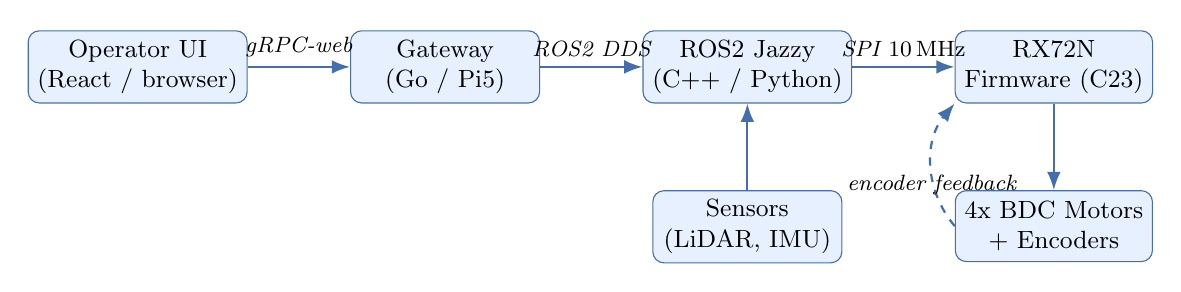
\begin{tikzpicture}[node distance=1.1cm and 1.3cm]
\node[sddbox] (ui)  {Operator UI\\(React / browser)};
\node[sddbox, right=of ui]  (gw)  {Gateway\\(Go / Pi5)};
\node[sddbox, right=of gw]  (ros) {ROS2 Jazzy\\(C++ / Python)};
\node[sddbox, right=of ros] (rx)  {RX72N\\Firmware (C23)};
\node[sddbox, below=of ros] (sen) {Sensors\\(LiDAR, IMU)};
\node[sddbox, below=of rx]  (mot) {4x BDC Motors\\+ Encoders};

\draw[sddarrow] (ui) -- node[above,sddlabel]{gRPC-web} (gw);
\draw[sddarrow] (gw) -- node[above,sddlabel]{ROS2 DDS} (ros);
\draw[sddarrow] (ros) -- node[above,sddlabel]{SPI \qty{10}{\mega\hertz}} (rx);
\draw[sddarrow] (sen) -- (ros);
\draw[sddarrow] (rx) -- (mot);
\draw[sddarrow, dashed] (mot.west) to[bend left=40] node[sddlabel,below]{encoder feedback} (rx.south west);
\end{tikzpicture}
\caption{STAR system context. Commands flow left to right; telemetry
flows right to left.}
\label{fig:system-context}
\end{figure}

\subsection{Deployment Topology}
The host computer is a Raspberry Pi 5 running Ubuntu 24.04 with ROS2
Jazzy installed from the OSRF apt repository. The gateway binary runs
as a systemd unit on the Pi5, bound to loopback for gRPC and to a
TLS-terminated Caddy reverse proxy for WebSocket and HTTP. The RX72N
is mounted on the custom motherboard PCB and communicates with the Pi5
via a dedicated SPI bus. Sensors attach to the Pi5 directly: the
RPLiDAR C1 over USB, the IMU over I2C through the RX72N's bus manager.

%======================================================================
% 4. Software Architecture
%======================================================================
\section{Software Architecture}
\label{sec:architecture}

\subsection{Architectural Style}
STAR is organized as a \emph{layered service-oriented hybrid}. The
layered aspect applies to the communication stack: the operator UI
sits above the gateway, which sits above ROS2, which sits above the
RX72N firmware. The service-oriented aspect applies horizontally
within each layer: the gateway is composed of five independent gRPC
services (motor control, telemetry, configuration, gateway control,
firmware update), and the ROS2 autonomy layer is composed of eight
packages that communicate only through DDS topics and actions.

Figure~\ref{fig:components} shows the eight software subsystems and
their principal dependencies.

\begin{figure}[H]
\centering
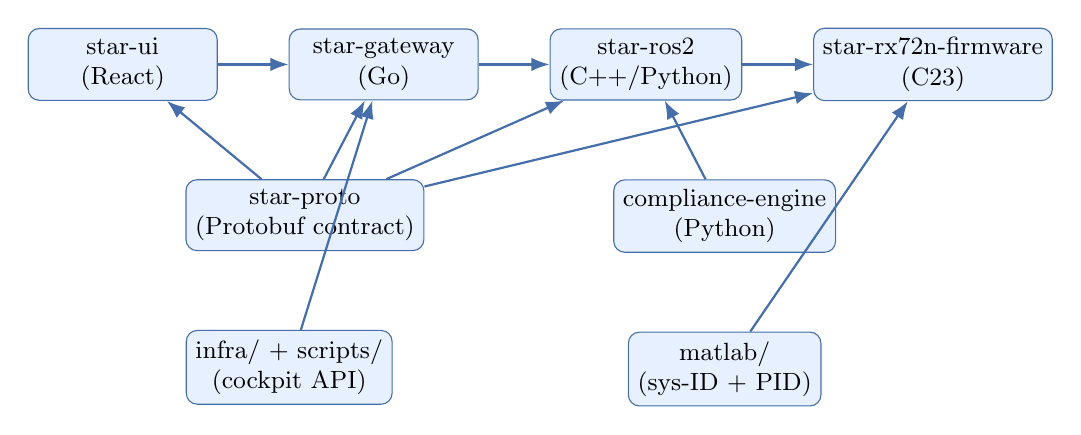
\begin{tikzpicture}[node distance=1.0cm and 0.9cm]
\node[sddbox] (ui) {star-ui\\(React)};
\node[sddbox, right=of ui] (gw) {star-gateway\\(Go)};
\node[sddbox, right=of gw] (ros) {star-ros2\\(C++/Python)};
\node[sddbox, right=of ros] (fw) {star-rx72n-firmware\\(C23)};

\node[sddbox, below=of gw, xshift=-1.0cm] (proto) {star-proto\\(Protobuf contract)};
\node[sddbox, below=of ros, xshift=1.0cm] (comp) {compliance-engine\\(Python)};

\node[sddbox, below=of proto, xshift=-0.2cm] (infra) {infra/ + scripts/\\(cockpit API)};
\node[sddbox, below=of comp]  (matlab) {matlab/\\(sys-ID + PID)};

\draw[sddarrow] (ui) -- (gw);
\draw[sddarrow] (gw) -- (ros);
\draw[sddarrow] (ros) -- (fw);
\draw[sddarrow] (proto) -- (ui);
\draw[sddarrow] (proto) -- (gw);
\draw[sddarrow] (proto) -- (ros);
\draw[sddarrow] (proto) -- (fw);
\draw[sddarrow] (comp) -- (ros);
\draw[sddarrow] (matlab) -- (fw);
\draw[sddarrow] (infra) -- (gw);
\end{tikzpicture}
\caption{Subsystem component diagram. Arrows denote
``depends on'' relationships at build time or runtime.}
\label{fig:components}
\end{figure}

\subsection{Subsystem Responsibilities}
The eight subsystems partition the codebase along clear responsibility
boundaries:

\begin{itemize}[leftmargin=1.4em,itemsep=2pt]
\item \textbf{star-proto} owns the language-neutral API contract and
      emits Go, TypeScript, C (nanopb), and C++ bindings.
\item \textbf{star-rx72n-firmware} owns hard-real-time motor control,
      encoder decoding, IMU reading, and SPI peripheral framing.
\item \textbf{star-gateway} owns the five-layer protocol stack and
      bridges the UI to both ROS2 and the RX72N.
\item \textbf{star-ros2} owns SLAM, sensor fusion, Nav2 planning,
      lifecycle-managed safety monitoring, and action servers.
\item \textbf{star-ui} owns all user-facing operator workflows:
      teleoperation, autonomy mode switching, telemetry plotting,
      compliance-report viewing.
\item \textbf{matlab} owns offline motor system identification and
      PID gain design; it exports gains to the firmware via a
      generated header.
\item \textbf{infra/ + scripts/} owns the Pi5 cockpit REST API, Caddy
      reverse-proxy configuration, and field-provisioning shell
      scripts.
\item \textbf{compliance-engine} owns the ADA 405.2 and related
      geometric audit checks running as ROS2 Python nodes.
\end{itemize}

\subsection{Cross-Cutting Concerns}
Five cross-cutting concerns are enforced across every subsystem:
\textbf{error handling} is return-value-based in C and Go (no
exceptions), exception-based in C++ ROS2 nodes, and Promise-based in
TypeScript; \textbf{logging} uses the native facility of each runtime
(\texttt{printf}-like \texttt{rx\_log\_*} on RX72N, structured logs in
Go, \texttt{RCLCPP\_*} in C++, a ring-buffer alert bus in React);
\textbf{unit convention} is MKS throughout with explicit suffixes
(\texttt{\_mps}, \texttt{\_rad}, \texttt{\_ma}, \texttt{\_celsius});
\textbf{character encoding} is 7-bit ASCII only, enforced at commit
time; and \textbf{memory allocation} on the RX72N is statically
bounded, with zero \texttt{malloc} or \texttt{free} calls after the
boot sequence.

%======================================================================
% 5. Component/Module Descriptions
%======================================================================
\section{Component and Module Descriptions}
\label{sec:component-descriptions}

This section describes each subsystem in turn. For each, we cover
purpose, internal modules, primary inputs and outputs, dependencies,
and key algorithmic logic.

\subsection{star-proto (API Contract)}
\textbf{Purpose:} Provide a single source of truth for all STAR
message and service definitions, and emit language bindings for the
four downstream runtimes.

\textbf{Inventory:} Ten Protocol Buffers files under
\texttt{star-proto/proto/star/v1/}: \texttt{common.proto},
\texttt{configuration.proto}, \texttt{controller.proto},
\texttt{diagnostics.proto}, \texttt{firmware\_update.proto},
\texttt{gateway\_service.proto}, \texttt{motor\_control.proto},
\texttt{telemetry.proto}, \texttt{ui.proto}, and \texttt{wire.proto}.

\textbf{Code generation:} Managed by the Buf CLI (version 1.28.1) via
\texttt{buf.gen.yaml}. Go bindings use
\texttt{buf.build/protocolbuffers/go} and
\texttt{buf.build/grpc/go}; TypeScript uses
\texttt{timostamm-protobuf-ts} (2.11.1); C bindings are generated by
\texttt{nanopb\_generator}; C++ bindings use the standard
\texttt{protoc-gen-cpp}.

\textbf{nanopb field sizing:} RX72N has no dynamic allocation, so
every variable-length field must declare a compile-time maximum via
an adjacent \texttt{.options} file. Example:
\texttt{star.v1.RequestHeader.request\_id max\_size:64}.

\textbf{Style:} Boston Dynamics Proto3 conventions:
\texttt{PascalCase} messages, \texttt{snake\_case} fields,
\texttt{SCREAMING\_SNAKE} enums with a zero value ending in
\texttt{\_UNKNOWN}, 100-character line limit, MKS unit suffixes, and a
\texttt{RequestHeader}/\texttt{ResponseHeader} pair on every RPC
message.

\subsection{star-rx72n-firmware (Real-Time Motor Control)}
\textbf{Purpose:} Provide deterministic closed-loop control of four
brushed DC gearmotors while serving as an SPI peripheral to the Pi5
gateway.

\textbf{Platform:} Renesas RX72N, 32-bit RX CPU core at
\qty{240}{\mega\hertz} (ICLK), \qty{4}{\mega\byte} Flash,
\qty{512}{\kilo\byte} SRAM, GNURX toolchain, CMake-driven build.

\textbf{RTOS:} Azure RTOS ThreadX with seven statically allocated
tasks, shown in Table~\ref{tab:threadx-tasks}.

\begin{table}[H]
\centering
\caption{ThreadX tasks on RX72N firmware.}
\label{tab:threadx-tasks}
\small
\begin{tabular}{l c c l}
\toprule
\textbf{Task} & \textbf{Priority} & \textbf{Stack} & \textbf{Role} \\
\midrule
CommTask            & P5  & \qty{2}{\kilo\byte}   & SPI framer, nanopb codec \\
MotorControlTask    & P12 & \qty{2}{\kilo\byte}   & 250 Hz PID servo \\
WatchdogMonitorTask & P20 & \qty{1}{\kilo\byte}   & RTOS + WDT health \\
ObstacleDetectTask  & P22 & \qty{1.5}{\kilo\byte} & Sonar + proximity fusion \\
TempSensorTask      & P24 & \qty{1}{\kilo\byte}   & BMP280 + thermistor \\
LEDStatusTask       & P25 & \qty{0.5}{\kilo\byte} & Status LED state machine \\
TelemetryTask       & P26 & \qty{1}{\kilo\byte}   & Diagnostics aggregation \\
\bottomrule
\end{tabular}
\end{table}

\textbf{HAL modules:} CMT (compare-match timer), GPTW (four channels
of \qty{20}{\kilo\hertz} motor PWM with \qty{1}{\micro\second} hardware
dead-time), TPU (quadrature encoder decoding at 341 PPR), RSPI (SPI
peripheral mode), SCI (debug UART through the CY7C65213 USB-UART
bridge), RIIC (BNO055 IMU and BMP280 barometer), hardware CRC-32
(polynomial \texttt{0xEDB88320}, approximately
\qty{32}{\micro\second} for 100 bytes), DMACA, MPC (multi-function pin
controller), WDT and IWDT, and the POEG port output-enable gate used
as an H-bridge fail-safe kill switch.

\textbf{Motor driver:} Each of four channels drives a DRV8263H dual
H-bridge in IN/IN PWM mode. The startup sequence is DRVOFF high,
\texttt{nSLEEP} high, wait \texttt{tWAKE}, then DRVOFF low.

\textbf{Library sizes (LOC):} \texttt{rx\_hal} 57.7k, \texttt{threadx}
43.5k, \texttt{rx\_core} 26.7k, \texttt{rx\_bus} 14.9k,
\texttt{rx\_nanopb} 7.2k, \texttt{rx\_spi\_comm} 4.2k,
\texttt{rx\_comm\_manager} 3.6k, \texttt{rx\_encoder} 3.4k,
\texttt{rx\_motor} 2.6k, \texttt{rx\_pid} 2.3k; roughly 71k LOC total
across the firmware libraries.

\textbf{Error convention:} \texttt{rx\_err\_t} is a signed 32-bit
integer. Code ranges: \texttt{0x000} success, \texttt{0x100--0x1FF}
generic, \texttt{0x200--0x2FF} hardware, \texttt{0x300--0x3FF} RTOS,
\texttt{0x400--0x4FF} communication, \texttt{0x500--0x5FF} validation.

\textbf{Boot budget at \qty{240}{\mega\hertz}:} Approximately
\qty{50}{\milli\second} from reset to \texttt{tx\_kernel\_enter()}
(reset-flag check, clock init, hardware init, USB enum, kernel start).

\subsection{star-gateway (Go Protocol Bridge)}
\textbf{Purpose:} Bridge between the operator UI and both the RX72N
SPI peripheral and the ROS2 autonomy layer. Runs as a systemd service
on the Pi5.

\textbf{Stack:} Go 1.26.2, \texttt{google.golang.org/grpc} v1.80.0,
\texttt{gorilla/websocket} for WebSocket transport to the UI, and
\texttt{periph.io} v3 for Linux SPI device access.

\textbf{Five-layer protocol stack} (from application down to
hardware): gRPC service handlers, Chase Combining HARQ retransmission,
rate-1/2 K=7 convolutional FEC, framing (sync + length + sequence +
CRC-32), SPI \qty{10}{\mega\hertz} (CPOL=0, CPHA=0) transport.

\textbf{gRPC services:} \texttt{MotorControlService},
\texttt{TelemetryService}, \texttt{ConfigurationService},
\texttt{GatewayService}, \texttt{FirmwareUpdateService}.

\textbf{Environment flags:} \texttt{WS\_STRICT\_ORIGIN} toggles
WebSocket origin checking, \texttt{STAR\_CDC\_DEVICE} selects the
USB-CDC fallback device for firmware flashing,
\texttt{STAR\_SIMULATION\_MODE} routes SPI traffic through an
in-process virtual RX72N, and \texttt{TRANSPORT\_MODE} selects
SPI, CDC, or simulated transport at startup.

\subsection{star-ros2 (Autonomy)}
\textbf{Purpose:} Perception, localization, mapping, path planning,
and safety monitoring.

\textbf{Distribution:} ROS2 Jazzy on Ubuntu 24.04, C++20 with
\texttt{rclcpp}, plus Python nodes where appropriate.

\textbf{Packages (10 total in \texttt{star-ros2/src/}):}
\texttt{star\_bringup} (launch orchestration),
\texttt{star\_simple\_bridge} (\statuslabel{IMPLEMENTED} -- the deployed
USB-CDC ASCII bridge to the RX72N at 115200~baud; serves
OccupancyGrid PNG and Prometheus metrics on \texttt{:9101}),
\texttt{star\_spi\_bridge} (\statuslabel{ARCHITECTED} -- the production
SPI bridge target; not used at defense),
\texttt{star\_gateway\_bridge}, \texttt{star\_safety\_monitor}
(lifecycle-managed emergency stop), \texttt{star\_perception}
(point-cloud preprocessing), \texttt{star\_simulation} (SITL harness),
\texttt{star\_supervisor} (top-level state coordinator),
\texttt{star\_compliance\_msgs} (custom message definitions for the
ADA compliance engine), and \texttt{sllidar\_ros2} (vendor driver for
the RPLiDAR C1).

\textbf{Third-party stack:} \texttt{slam\_toolbox} (async SLAM with
loop closure), \texttt{robot\_localization} (EKF fusing
\texttt{/odom/unfiltered} with \texttt{/imu/data}), Nav2 for
occupancy-grid path planning, and \texttt{explore\_lite} for frontier
exploration.

\textbf{TF tree:} \texttt{map -> odom -> base\_link -> \{laser\_frame,
imu\_link\}} following REP-105.

\subsection{star-ui (Operator Dashboard)}
\textbf{Purpose:} Provide a single-page browser application for
teleoperation, autonomy mode selection, live telemetry plotting, and
compliance-report viewing.

\textbf{Stack:} React 19.2.0, TypeScript 5.9, Vite 7.2.4 (build),
Zustand 5.0.3 (state), uPlot 1.6.31 (GPU-accelerated time-series
plots), \texttt{react-grid-layout} (dashboard panel placement), and
gRPC-web (telemetry streams and command unary RPCs).

\textbf{Panel inventory:} Seventeen panels, including live map view,
command velocity joystick, four motor plots, IMU orientation display,
LiDAR scan overlay, alert log ring buffer, autonomy mode switch,
emergency-stop panel, SLAM control, firmware-update panel, and the
compliance-report viewer.

\textbf{Reconnection:} WebSocket transport implements exponential
backoff reconnection with jitter; the frontend degrades gracefully to
``stale'' indicators after the first reconnect attempt exceeds one
second.

\subsection{matlab (Motor System Identification and PID Design)}
\textbf{Purpose:} Offline identification of the motor-plant transfer
function from step-response data, and deterministic computation of PID
gains that satisfy the firmware's real-time constraints.

\textbf{Identified plant:} The open-loop transfer function from input
voltage to angular velocity is
\[
  G(s) = \frac{3.665}{0.075 s + 1}
\]
a first-order model with DC gain \qty{3.665}{\radian\per\second\per\volt}
and mechanical time constant $\tau = \qty{0.075}{\second}$
(\qty{75}{\milli\second}). The identification is performed in the
MATLAB System Identification Toolbox on a step-response data set
captured at the \qty{250}{\hertz} firmware sample rate.

\textbf{Validation plots:} The MATLAB workflow produces three
validation figures. The first overlays measured versus modeled
step response and demonstrates that the closed-loop response settles
within two seconds with an overshoot under ten percent for the tuned
gains. The second is a Bode plot showing a flat low-frequency
magnitude asymptote at the identified DC gain and a single real-pole
rolloff at approximately \qty{13.3}{\radian\per\second}
(equal to $1/\tau$ with $\tau = \qty{0.075}{\second}$). The third is a
closed-loop disturbance-rejection plot, confirming that the chosen
gains reject a simulated load step without oscillatory return. The
plot set constitutes the go/no-go checkpoint before new gains are
exported to the firmware.

\textbf{Why offline:} Three reasons. First, safety: autotuning on
hardware with untrusted gains risks winding the motor against
mechanical stops. Second, reproducibility: the MATLAB script
deterministically produces the same gains from the same data, which
allows regression review across semesters. Third, export determinism:
gains are written via \texttt{pid\_config\_output.txt} into a header
consumed by the firmware build, so a rebuild is the only coupling
between controller design and deployed code.

\subsection{infra/ and scripts/ (Pi5 Cockpit)}
\textbf{Purpose:} Minimal facility for operators to observe and
control the Pi5 host itself, independent of ROS2.

\textbf{Stack:} Python 3 Flask service at \texttt{:9102}, which
imports \texttt{rclpy} for read-only ROS2 introspection. Caddy is
fronted on port 443 with a local certificate authority for
development. Systemd unit files run both Caddy and the cockpit API
with sandbox directives
(\texttt{NoNewPrivileges}, \texttt{PrivateTmp}, \texttt{ProtectSystem}).

\textbf{Endpoints:} \texttt{/api/state} (aggregate health status),
\texttt{/api/autonomy/toggle}, \texttt{/api/estop/toggle}, and the
\texttt{/api/slam/*} family for start, stop, and map save.

\textbf{Scripts:} \texttt{scripts/} carries provisioning, build,
flash, and maintenance automation in Bash and Python, all under
pre-commit-enforced 7-bit ASCII.

\subsection{Compliance Engine (ADA Audit Core)}
\label{sec:compliance-engine}

\phantomsection
\label{sec:status-legend}
\textbf{Status-label legend (applies throughout this document; every
\texttt{[IMPLEMENTED]} / \texttt{[STRETCH]} / \texttt{[ARCHITECTED]}
tag elsewhere in the SDD links back here):}
\emph{[IMPLEMENTED]} means the feature is complete and has passing
tests; \emph{[STRETCH]} means a working stub with scaffolding in place
but without the full algorithm; \emph{[ARCHITECTED]} means specified
and designed but not yet coded.

\textbf{Purpose:} Apply ADA 405.2 and neighboring geometric checks to
fused point-cloud, odometry, and IMU data and emit a structured
compliance report.

\textbf{Stack:} Python 3, ROS2 \texttt{rclpy} nodes under
\texttt{final\_capstone/compliance-engine/}, packaged with
\texttt{setuptools} and \texttt{ament\_python}. Numerical work uses
Open3D and NumPy.

\textbf{Checks:} all eleven nodes below ship as files under
\texttt{final\_capstone/compliance-engine/star\_compliance/nodes/};
the status label tracks the algorithmic completeness of each.
\begin{itemize}[leftmargin=1.4em,itemsep=2pt]
\item \textbf{Ramp slope} (\texttt{ramp\_slope\_node.py}) --
      \statuslabel{IMPLEMENTED}. RANSAC plane fit to LiDAR points in a
      ramp region of interest, cross-validated against RX72N IMU pitch.
\item \textbf{Trip hazard} (\texttt{trip\_hazard\_node.py}) --
      \statuslabel{STRETCH stub}. Detects vertical discontinuities above
      the ADA threshold (one quarter inch).
\item \textbf{Path width} (\texttt{path\_width\_node.py}) --
      \statuslabel{STRETCH stub}. Occupancy-grid cross-section width
      along the planned path.
\item \textbf{Ramp width} (\texttt{ramp\_width\_node.py}),
      \textbf{ramp landing} (\texttt{ramp\_landing\_node.py}),
      \textbf{door clear width} (\texttt{door\_clear\_width\_node.py}),
      \textbf{door threshold} (\texttt{door\_threshold\_node.py}),
      \textbf{path blockage} (\texttt{path\_blockage\_node.py}),
      \textbf{protruding objects} (\texttt{protruding\_objects\_node.py}),
      \textbf{dynamic obstacle} (\texttt{dynamic\_obstacle\_node.py}),
      and the supervising \textbf{compliance monitor}
      (\texttt{compliance\_monitor\_node.py}) -- \statuslabel{ARCHITECTED stubs}.
      Node skeletons, message schemas, and traceability-matrix rows
      are committed to the repo; the internal algorithm bodies are
      placeholders pending post-capstone work.
\end{itemize}

\textbf{Core engines:} \texttt{engines/plane\_segmentation.py}
implements the RANSAC plane extractor used by the ramp checks, and
\texttt{engines/imu\_cross\_validate.py} reconciles the measured
plane slope against IMU pitch to flag suspected sensor drift.

\textbf{Reporting:} The \texttt{report/} package generates a PDF
audit report; an example is stored at
\texttt{star\_audit\_report\_sample.pdf}. Structured per-check
messages are published on \texttt{/compliance/report} and the
per-check topics enumerated in Section~\ref{sec:interfaces}.

\textbf{Tests:} \texttt{compliance-engine/tests/} contains
\texttt{pytest} unit tests for the engines and a small set of
golden-output integration tests. The traceability matrix at
\texttt{final\_capstone/extras/traceability.md} maps every ADA check
row to its sensor, algorithm, node, output topic, and status label,
and is reproduced in Appendix~\ref{sec:traceability}.

%======================================================================
% 6. Data Design
%======================================================================
\section{Data Design}
\label{sec:data-design}

\subsection{Protocol Buffers Schema Inventory}
The ten proto files under \texttt{star-proto/proto/star/v1/} are
summarized in Table~\ref{tab:proto-inventory}.

\begin{table}[H]
\centering
\caption{Protocol Buffers file inventory.}
\label{tab:proto-inventory}
\small
\begin{tabularx}{\linewidth}{l X}
\toprule
\textbf{File} & \textbf{Role} \\
\midrule
\texttt{common.proto}           & Shared envelopes (RequestHeader,
                                  ResponseHeader, Status) \\
\texttt{configuration.proto}    & PID and calibration payloads \\
\texttt{controller.proto}       & Operator command messages \\
\texttt{diagnostics.proto}      & Health and telemetry diagnostics \\
\texttt{firmware\_update.proto} & Firmware image + CRC metadata \\
\texttt{gateway\_service.proto} & Gateway control RPCs \\
\texttt{motor\_control.proto}  & Per-motor commands + feedback \\
\texttt{telemetry.proto}        & Streaming telemetry schema \\
\texttt{ui.proto}               & UI-specific envelopes \\
\texttt{wire.proto}             & Transport-layer framing types \\
\bottomrule
\end{tabularx}
\end{table}

\subsection{Wire Frame Layout}
Table~\ref{tab:wire-frame} describes the physical frame on the SPI
wire between the Pi5 and the RX72N.

\begin{table}[H]
\centering
\caption{SPI wire-frame layout (little-endian on the wire).}
\label{tab:wire-frame}
\small
\begin{tabular}{l c l}
\toprule
\textbf{Field} & \textbf{Size (bytes)} & \textbf{Description} \\
\midrule
Sync    & 2 & Fixed pattern \texttt{0xA55A} \\
Length  & 2 & Payload byte count, unsigned \\
Seq     & 2 & Monotonic sequence number, wraps \\
Payload & N & Nanopb-encoded protobuf message \\
CRC-32  & 4 & Polynomial \texttt{0xEDB88320} over Length..Payload \\
\bottomrule
\end{tabular}
\end{table}

\subsection{UI State Shape}
The React operator dashboard uses a single Zustand store split into
four top-level slices: \texttt{connection} (transport health,
reconnect state), \texttt{telemetry} (motor, IMU, battery),
\texttt{autonomy} (Nav2 state, SLAM state), and \texttt{alerts} (a
200-entry capped ring buffer of UI and transport alerts). Each slice
is serializable for debug export.

\subsection{ROS2 Topic and TF Graph}
The canonical topic set is listed in Section~\ref{sec:interfaces}
Table~\ref{tab:ros2-topics}. The transform tree follows REP-105 with
\texttt{map -> odom -> base\_link}, and \texttt{base\_link} parents
the two sensor frames \texttt{laser\_frame} and \texttt{imu\_link}.

\subsection{Compliance Report Schema}
Each compliance run emits a \texttt{ComplianceReport} message
containing a facility identifier, a run timestamp, and a list of
\texttt{CheckResult} entries. A \texttt{CheckResult} carries the
check identifier (for example, \texttt{ADA\_405\_2\_RAMP\_SLOPE}), the
measured value, the ADA threshold, a pass / fail / insufficient-data
verdict, and a sensor-provenance record.

\subsection{Protocol-Stack Data Flow}
Figure~\ref{fig:protocol-stack} traces the transmit path from an
operator action in the UI down to the electrical SPI signals on the
RX72N pins. The receive path mirrors this diagram in reverse.

\begin{figure}[H]
\centering
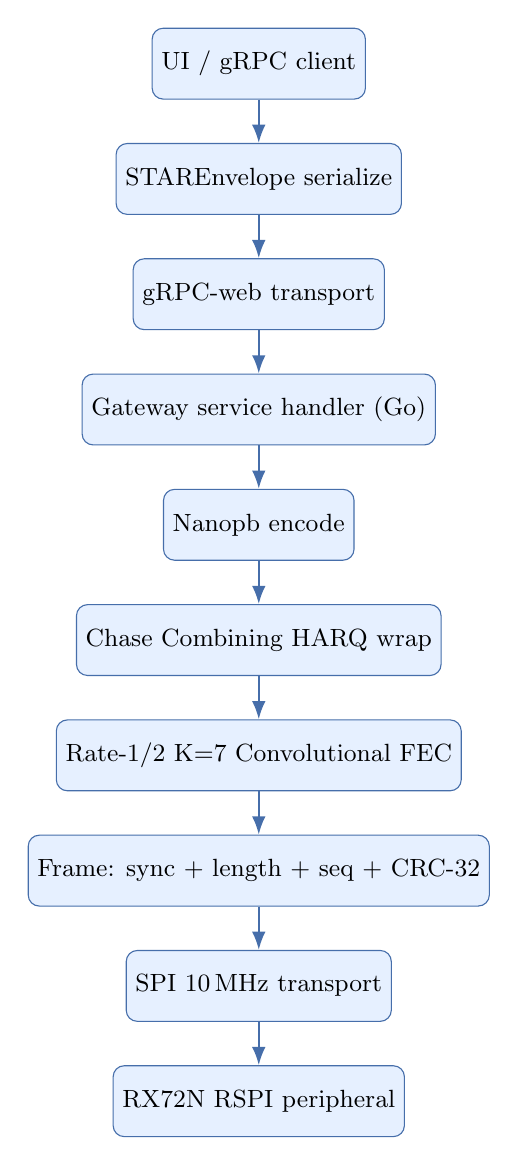
\begin{tikzpicture}[node distance=0.55cm, every node/.style={font=\small}]
\node[sddbox] (app)   {UI / gRPC client};
\node[sddbox, below=of app]   (env)  {STAREnvelope serialize};
\node[sddbox, below=of env]   (web)  {gRPC-web transport};
\node[sddbox, below=of web]   (svc)  {Gateway service handler (Go)};
\node[sddbox, below=of svc]   (np)   {Nanopb encode};
\node[sddbox, below=of np]    (hq)   {Chase Combining HARQ wrap};
\node[sddbox, below=of hq]    (fec)  {Rate-1/2 K=7 Convolutional FEC};
\node[sddbox, below=of fec]   (fr)   {Frame: sync + length + seq + CRC-32};
\node[sddbox, below=of fr]    (spi)  {SPI \qty{10}{\mega\hertz} transport};
\node[sddbox, below=of spi]   (rspi) {RX72N RSPI peripheral};

\draw[sddarrow] (app) -- (env);
\draw[sddarrow] (env) -- (web);
\draw[sddarrow] (web) -- (svc);
\draw[sddarrow] (svc) -- (np);
\draw[sddarrow] (np) -- (hq);
\draw[sddarrow] (hq) -- (fec);
\draw[sddarrow] (fec) -- (fr);
\draw[sddarrow] (fr) -- (spi);
\draw[sddarrow] (spi) -- (rspi);
\end{tikzpicture}
\caption{Protocol-stack data flow (transmit path, top-to-bottom).
The receive path mirrors this diagram in reverse. HARQ and FEC sit
below the gRPC transport on the transmit side; they are not wrapped
around gRPC.}
\label{fig:protocol-stack}
\end{figure}

%======================================================================
% 7. Interface Design
%======================================================================
\section{Interface Design}
\label{sec:interfaces}

\subsection{SPI Physical Layer}
Shared bus between the Pi5 controller and the RX72N peripheral. Clock
rate \qty{10}{\mega\hertz}, CPOL = 0, CPHA = 0, MSB-first, 8-bit word.
Chip select is driven by a single GPIO on the Pi5. The Pi5 side uses
the \texttt{periph.io} SPI driver, and the RX72N side uses RSPI in
peripheral mode with DMA-backed ping-pong buffers.

\subsection{gRPC Services}
Five services are defined in the proto inventory. Every request
carries a \texttt{RequestHeader} and every response carries a
\texttt{ResponseHeader}.

\begin{itemize}[leftmargin=1.4em,itemsep=2pt]
\item \texttt{MotorControlService} -- \texttt{SetVelocity},
      \texttt{SetPosition}, \texttt{EmergencyStop},
      \texttt{GetMotorStatus}.
\item \texttt{TelemetryService} -- \texttt{StreamTelemetry} (server
      streaming), \texttt{SnapshotTelemetry} (unary).
\item \texttt{ConfigurationService} -- \texttt{GetConfig},
      \texttt{SetConfig}, \texttt{CommitConfig}.
\item \texttt{GatewayService} -- \texttt{Ping}, \texttt{GetStatus},
      \texttt{Restart}, \texttt{SwitchTransport}.
\item \texttt{FirmwareUpdateService} -- \texttt{StartUpdate},
      \texttt{StreamImage}, \texttt{FinalizeUpdate}.
\end{itemize}

\subsection{WebSocket Binary Envelope}
The UI connects to the gateway using a WebSocket upgrade on top of
Caddy TLS. All frames are binary (opcode 2) and carry a single
\texttt{STAREnvelope} message. The envelope discriminates between
telemetry frames, alert frames, and command frames by a tagged oneof.

\subsection{ROS2 Topic Inventory}
Table~\ref{tab:ros2-topics} lists the canonical ROS2 topics that
cross package boundaries, including all compliance-engine topics.

\begin{table}[H]
\centering
\caption{ROS2 canonical topic inventory.}
\label{tab:ros2-topics}
\small
\begin{tabularx}{\linewidth}{l l X}
\toprule
\textbf{Topic} & \textbf{Type} & \textbf{Role} \\
\midrule
\texttt{/cmd\_vel}                   & \texttt{geometry\_msgs/Twist} & Velocity command \\
\texttt{/odom/unfiltered}            & \texttt{nav\_msgs/Odometry}   & Wheel odometry pre-fusion \\
\texttt{/odom/filtered}              & \texttt{nav\_msgs/Odometry}   & EKF output \\
\texttt{/imu/data}                   & \texttt{sensor\_msgs/Imu}     & BNO055 fused IMU \\
\texttt{/scan}                       & \texttt{sensor\_msgs/LaserScan} & RPLiDAR C1 scan \\
\texttt{/map}                        & \texttt{nav\_msgs/OccupancyGrid} & SLAM output \\
\texttt{/diagnostics}                & \texttt{diagnostic\_msgs/...} & Health aggregator \\
\texttt{/compliance/report}          & \texttt{star\_msgs/Report}    & Aggregate audit result \\
\texttt{/compliance/ramp\_slope}     & \texttt{star\_msgs/Check}     & Per-check result \\
\texttt{/compliance/trip\_hazard}    & \texttt{star\_msgs/Check}     & Per-check result \\
\texttt{/compliance/path\_width}     & \texttt{star\_msgs/Check}     & Per-check result \\
\bottomrule
\end{tabularx}
\end{table}

\subsection{Pi5 Cockpit REST API}
Four primary REST endpoints are exposed by the Flask cockpit on
\texttt{:9102} behind Caddy TLS: \texttt{/api/state} (GET, aggregate
health), \texttt{/api/autonomy/toggle} (POST, toggle autonomy mode),
\texttt{/api/estop/toggle} (POST, engage or clear emergency stop),
and \texttt{/api/slam/\{start,stop,save\}} (POST).

\subsection{UI Panel Inventory}
The seventeen React panels include: live 2D map, LiDAR overlay,
joystick teleoperation, four per-motor live plots (one per wheel),
IMU orientation, battery, temperature, alert log, autonomy mode
switch, emergency stop, SLAM control, firmware update, compliance
summary, compliance per-check, system health, and a diagnostic raw
log panel for debugging.

%======================================================================
% 8. Technology Stack
%======================================================================
\section{Technology Stack and Justifications}
\label{sec:tech-stack}

Table~\ref{tab:stack} enumerates the technology choices made for the
STAR software project, together with a short justification. Version
numbers are pinned by the top-level lockfiles and package manifests.

\begin{table}[H]
\centering
\caption{Technology stack and selection rationale.}
\label{tab:stack}
\small
\begin{tabularx}{\linewidth}{l l X}
\toprule
\textbf{Subsystem} & \textbf{Choice} & \textbf{Rationale} \\
\midrule
Gateway             & Go 1.26.2             & First-class gRPC, small binaries, cgo-free SPI via periph.io \\
Firmware            & C23, GNURX, ThreadX   & Vendor toolchain support, C23 typed enums, small RTOS footprint \\
ROS2 distribution   & Jazzy (Ubuntu 24.04)  & Long-term support release matched to rclcpp C++20 \\
UI framework        & React 19.2 + Vite 7   & Concurrent rendering, fast HMR, mature component ecosystem \\
UI state            & Zustand 5.0.3         & Minimal API, no boilerplate, selector memoization \\
UI plots            & uPlot 1.6.31          & GPU-friendly time-series plots, tiny bundle \\
Proto build         & Buf 1.28.1            & Reproducible lint and breaking-change detection \\
TypeScript bindings & protobuf-ts 2.11.1    & First-class gRPC-web, clean TS ergonomics \\
C bindings          & nanopb                & Zero dynamic allocation, proto3 subset \\
Compliance nodes    & rclpy (Python 3)      & NumPy/Open3D access, rapid iteration on algorithms \\
MATLAB              & Control + System ID   & Canonical offline sys-ID and PID design workflow \\
Reverse proxy       & Caddy                 & Automatic TLS with local CA, small config surface \\
Cockpit API         & Flask + rclpy         & Single-file REST, trivial systemd integration \\
\bottomrule
\end{tabularx}
\end{table}

Specific reasons for non-obvious choices:

\textbf{Why ThreadX over FreeRTOS?} Renesas distributes vetted
ThreadX ports for the RX72N with guaranteed memory footprints. The
static-allocation discipline aligns naturally with NASA Power of 10
Rule 3.

\textbf{Why Buf over \texttt{protoc} directly?} Buf enforces style
rules, detects breaking changes on every push, and produces
reproducible generated artifacts across CI runners.

\textbf{Why protobuf-ts instead of ts-proto?} Better gRPC-web
support, cleaner oneof ergonomics, and an active maintainer
release cadence.

\textbf{Why rclpy for compliance, not C++?} The compliance engine is
algorithmically dominated by point-cloud work (Open3D, NumPy) where
Python has mature bindings, and real-time constraints do not apply:
compliance runs at mission cadence, not loop cadence.

%======================================================================
% 9. Key Algorithms and Logic
%======================================================================
\section{Key Algorithms and Logic}
\label{sec:algorithms}

\subsection{Cascaded PID (Position Outer, Velocity Inner)}
Each motor is controlled by a two-stage cascade. The outer position
loop produces a velocity setpoint; the inner velocity loop produces a
voltage setpoint that becomes a PWM duty ratio. In continuous time
each stage is a standard PID:
\[
  u(t) \;=\; K_p\, e(t) \;+\; K_i \int_0^t e(\tau)\, d\tau
         \;+\; K_d\, \frac{d e(t)}{d t}.
\]
In firmware we use the velocity form of the PID at sample period
$T_s = \qty{0.004}{\second}$ (\qty{250}{\hertz}):
\[
  u[k] = u[k-1] + K_p (e[k] - e[k-1]) + K_i T_s\, e[k]
       + \tfrac{K_d}{T_s} \bigl(e[k] - 2 e[k-1] + e[k-2]\bigr).
\]
The equivalent discrete transfer function is
\[
  C(z) = \frac{b_0 + b_1 z^{-1} + b_2 z^{-2}}{1 - z^{-1}}.
\]
Anti-windup uses integral clamping to the configured saturation
bounds; the derivative term is low-pass-filtered to limit sensor noise
amplification.

\begin{lstlisting}[style=pseudocode, caption={Velocity-form PID update.}, label={lst:pid}]
function pid_update(state, setpoint, measured, dt):
    e[k]   <- setpoint - measured
    du     <- Kp*(e[k] - state.e_km1)
            + Ki*dt*e[k]
            + (Kd/dt)*(e[k] - 2*state.e_km1 + state.e_km2)
    u_new  <- clamp(state.u_prev + du, u_min, u_max)
    state.e_km2 <- state.e_km1
    state.e_km1 <- e[k]
    state.u_prev <- u_new
    return u_new
\end{lstlisting}

\subsection{Quadrature Encoder Decoding}
The TPU peripheral is configured as a signed up/down counter clocked
by quadrature-decoded A/B edges. At each control tick the firmware
reads the counter, computes a signed delta modulo $2^{16}$ to handle
wraparound, and multiplies by the calibrated
\qty{1}{\text{count}}-to-radian conversion (341 PPR, 4x decoded = 1364
edges per revolution, and an optional gearbox ratio).

\subsection{Convolutional FEC and Viterbi Decoding}
The gateway applies a rate-1/2 convolutional encoder with constraint
length $K = 7$ and generator polynomials $G_1 = \texttt{171}_8$,
$G_2 = \texttt{133}_8$. The decoder runs soft-decision Viterbi with a
traceback depth of 35 (5K rule of thumb). Soft bits from the SPI
front-end are quantized to four bits per symbol before entering the
branch-metric accumulator.

\subsection{Chase Combining HARQ}
On a CRC failure the receiver retains the soft-bit vector for the
failed frame, and on retransmission the soft bits are added
elementwise before Viterbi decoding. This provides approximately
\qty{3}{\decibel} of combining gain after a single retransmission
and monotonically improves with further retransmissions up to the
configured cap.

\subsection{Sensor Fusion (robot\_localization EKF)}
\texttt{robot\_localization} runs an extended Kalman filter at
\qty{50}{\hertz} fusing wheel odometry (pose and twist) with IMU
orientation and angular-rate channels. The output is published on
\texttt{/odom/filtered} and consumed by SLAM and Nav2.

\subsection{SLAM and Exploration}
\texttt{slam\_toolbox} in asynchronous mode builds the occupancy grid
from the LiDAR scan, with pose-graph optimization performing loop
closure when revisiting landmarks. \texttt{explore\_lite} selects
frontier cells (occupancy-grid boundaries between known-free and
unknown cells) as the next navigation goal until no unexplored
frontier remains.

\subsection{WebSocket Reconnection}
The UI wraps its WebSocket in an exponential-backoff reconnect loop:
delay $d_n = \min(d_{max}, d_0 \cdot 2^n) + \text{jitter}$ with
$d_0 = \qty{250}{\milli\second}$, $d_{max} = \qty{15}{\second}$, and
jitter drawn uniformly from
\qtyrange{0}{250}{\milli\second}.

\subsection{RANSAC Plane Segmentation for ADA 405.2}
The compliance engine extracts the dominant plane from a LiDAR point
cloud using RANSAC: it samples three random points, fits a plane,
scores the plane by the count of inliers within a configured
tolerance, and iterates up to a bounded number of samples. The final
plane's normal vector determines the slope relative to gravity
(cross-checked against the IMU pitch). Pseudocode appears in
Listing~\ref{lst:ransac}.

\begin{lstlisting}[style=pseudocode, caption={RANSAC plane fit for ramp slope.}, label={lst:ransac}]
function ransac_plane(points, tol, n_iter):
    best_plane  <- null
    best_inliers <- 0
    for i in 1..n_iter:
        sample  <- random_choice(points, 3)
        plane   <- plane_from_three_points(sample)
        inliers <- count(p in points where dist(p, plane) < tol)
        if inliers > best_inliers:
            best_inliers <- inliers
            best_plane   <- plane
    return best_plane
\end{lstlisting}

%======================================================================
% 10. Error Handling and Logging
%======================================================================
\section{Error Handling and Logging}
\label{sec:errors}

\subsection{Error Propagation}
The RX72N firmware uses \texttt{rx\_err\_t} (signed 32-bit) return
codes exclusively; no C++ exceptions cross the RTOS boundary.
Propagation uses the \texttt{RX\_RETURN\_ON\_ERROR} macro, which
inspects the return value, logs a tagged error, and early-returns
if nonzero.

The Go gateway uses the standard \texttt{fmt.Errorf("context: \%w",
err)} wrap idiom and converts to gRPC status codes at service
boundaries using \texttt{status.Code}.

The ROS2 C++ layer propagates exceptions within a node and converts
them to lifecycle transitions or \texttt{/diagnostics} publications
at node boundaries.

The UI surfaces errors through a ring-buffer alert log capped at 200
entries; overflow discards the oldest entries. Each alert carries a
severity (info, warning, error), a tag, a timestamp, and an optional
structured payload.

\subsection{Logging Conventions}
\begin{itemize}[leftmargin=1.4em,itemsep=2pt]
\item RX72N: \texttt{rx\_log\_error}, \texttt{rx\_log\_warn},
      \texttt{rx\_log\_info}, \texttt{rx\_log\_debug}; level-gated at
      compile time via \texttt{LOG\_LEVEL}.
\item Go: structured logs via the standard \texttt{log/slog} package,
      with a JSON handler in production.
\item ROS2: \texttt{RCLCPP\_INFO}, \texttt{RCLCPP\_WARN},
      \texttt{RCLCPP\_ERROR} with per-node named loggers.
\item UI: the Zustand \texttt{alerts} slice plus a dev-only
      \texttt{console.debug} channel.
\end{itemize}

\subsection{Watchdog Strategy}
Both WDT and IWDT are enabled on the RX72N. The
\texttt{WatchdogMonitorTask} feeds the WDT and verifies that every
ThreadX task has checked in within a configured timeout. Missed
check-ins escalate to a POEG-driven H-bridge shutdown, which stops
the motors within microseconds.

%======================================================================
% 11. Security Considerations
%======================================================================
\section{Security Considerations}
\label{sec:security}

\subsection{WebSocket Origin and Transport}
The gateway defaults to \texttt{WS\_STRICT\_ORIGIN=true}, which
rejects WebSocket upgrades whose \texttt{Origin} header is not on
the allowlist. The operator UI is served over HTTPS by Caddy with a
locally generated certificate authority; the operator browser is
expected to trust that CA during field operation.

\subsection{gRPC Surface}
gRPC listens only on the loopback interface. Cross-host traffic to
the UI terminates at Caddy and is multiplexed over the WebSocket
binary envelope; gRPC-web calls from the UI are proxied to loopback
gRPC by the gateway.

\subsection{Firmware Update Integrity}
Firmware images are CRC-32-checked before and after transfer to the
RX72N. A signature field is reserved in \texttt{firmware\_update.proto}
for future cryptographic signing but is not yet enforced (see
Section~\ref{sec:limitations}).

\subsection{Service Sandboxing}
The cockpit API and gateway systemd units use
\texttt{NoNewPrivileges=true}, \texttt{PrivateTmp=true},
\texttt{ProtectSystem=strict}, and a restricted \texttt{ReadWritePaths}
set so the services cannot modify anything outside their state
directory.

\subsection{Character Encoding as Defense}
The 7-bit ASCII enforcement hook prevents the introduction of
confusable Unicode characters, homograph attacks in identifiers, and
smuggled payloads in string literals.

%======================================================================
% 12. Performance Considerations
%======================================================================
\section{Performance Considerations}
\label{sec:performance}

\subsection{Real-Time Budgets}
\begin{itemize}[leftmargin=1.4em,itemsep=2pt]
\item Motor control loop: \qty{250}{\hertz} servo
      (\qty{4}{\milli\second} period); PID math completes in
      approximately \qty{2}{\micro\second} at 240 MHz with \texttt{-O2}.
\item Watchdog monitor: feeds WDT at \qty{100}{\hertz}
      (\qty{10}{\milli\second} period).
\item SPI link budget: \qty{10}{\mega\hertz} raw,
      \qty{10}{\mega\bit\per\second} wire throughput; after rate-1/2
      FEC and framing the useful payload is approximately
      \qty{4.5}{\mega\bit\per\second} sustained.
\item Hardware CRC-32: approximately \qty{32}{\micro\second} per 100
      bytes on the RX72N hardware CRC peripheral.
\item ROS2 EKF: \qty{50}{\hertz} cycle.
\item UI rendering: 60 Hz via uPlot with GPU-accelerated canvas draws.
\end{itemize}

\subsection{Known Bottlenecks}
LiDAR USB jitter can spike scan latency to tens of milliseconds under
contention; the SLAM async pipeline absorbs this. ROS2 DDS discovery
storms can transiently saturate loopback on bringup; this is contained
by a staggered launch sequence in \texttt{star\_bringup}.

\subsection{Scalability Limits}
The current firmware supports exactly four motors, sized to the
available GPTW channels and dead-time generators. SRAM usage is
bounded statically and the margin at link time is less than
\qty{5}{\percent} of the \qty{512}{\kilo\byte} total; adding a fifth
motor would require pruning the debug logging buffer or upgrading to a
larger-SRAM RX variant.

%======================================================================
% 13. Testing Strategy
%======================================================================
\section{Testing Strategy}
\label{sec:testing}

\subsection{Unit Tests}
\begin{itemize}[leftmargin=1.4em,itemsep=2pt]
\item RX72N firmware: Unity v2.6.1 auto-fetched by CMake;
      approximately 35 test executables. Mocks cover
      \texttt{bus\_interface}, \texttt{motor},
      \texttt{uart}, \texttt{error\_handler}, and ThreadX
      primitives via \texttt{MOCK\_TX\_THREAD\_CREATE}.
\item Gateway: Go's built-in \texttt{testing} plus
      \texttt{testify} for nanopb bounds, frame codec, FEC, and
      Viterbi.
\item UI: Vitest plus \texttt{@testing-library/react} for components
      and Zustand slice reducers.
\item Compliance engine: \texttt{pytest} for the engines and golden
      outputs for the report generator.
\end{itemize}

\subsection{Integration Tests}
A \texttt{virtual\_rx72n} simulator reimplements the RX72N SPI
peripheral surface in-process so the gateway can execute end-to-end
protocol tests without hardware. ROS2 launch tests exercise startup
orchestration; gRPC conformance tests exercise the service surface.

\subsection{Hardware Bring-Up}
Dedicated bring-up executables live in the firmware tree:
\texttt{motor\_spin\_test/}, \texttt{pwm\_test/},
\texttt{encoder\_test/}, \texttt{gpio\_test/}, \texttt{uart\_test/},
\texttt{imu\_test/}, and \texttt{sonar\_test/}. These are built by
the firmware CMake presets and flashed individually.

\subsection{CI/CD}
GitHub Actions orchestrates all builds: firmware, gateway, UI, ROS2
(via Docker), and MATLAB linting. Pre-commit hooks enforce 7-bit
ASCII and basic formatting; CodeRabbit performs AI code review on
every pull request.

%======================================================================
% 14. Known Limitations and Future Work
%======================================================================
\section{Known Limitations and Future Work}
\label{sec:limitations}

\begin{itemize}[leftmargin=1.4em,itemsep=2pt]
\item \textbf{Four-motor ceiling.} Firmware is sized to exactly four
      GPTW PWM channels and four TPU encoder channels. A fifth motor
      requires hardware expansion.
\item \textbf{Single-robot SLAM.} \texttt{slam\_toolbox} supports only
      a single robot in the current configuration. Multi-robot
      deployments would require cooperative SLAM stacks such as
      Kimera-Multi or Swarm-SLAM.
\item \textbf{Global planner A* only.} Nav2 is configured with its
      default A* grid planner. More sophisticated planners such as
      Hybrid A* or state-lattice planners are future work for
      non-rectilinear environments.
\item \textbf{Firmware update signing.} The firmware-update path
      verifies CRC-32 only. Reserving a signature field in the proto
      is a first step; full signed-update verification with a
      public-key store on the RX72N is future work.
\item \textbf{Single-operator UI.} The dashboard assumes one
      operator; multi-operator arbitration, role separation, and
      audit logging are not implemented.
\item \textbf{PID gain design requires an offline MATLAB re-run for
      any plant model change; no online autotuning.} If the motor
      or the load changes significantly, the MATLAB workflow must be
      re-executed and the firmware rebuilt. STAR does not perform
      online PID autotuning.
\item \textbf{English-only UI.} Internationalization and
      localization infrastructure (i18n bundles, RTL layout) are not
      present.
\item \textbf{Compliance coverage.} Only the ramp-slope check is
      fully implemented; path width and trip hazard are stubs and
      the remaining ADA checks are specified but not coded.
\end{itemize}

%======================================================================
% 15. Appendices
%======================================================================
\section*{Appendices}
\addcontentsline{toc}{section}{Appendices}

\subsection*{Appendix A: Glossary}
\label{sec:glossary}
\addcontentsline{toc}{subsection}{Appendix A: Glossary}

\begin{description}[leftmargin=4em,style=nextline]
\item[RX72N]
A Renesas 32-bit microcontroller with a 240 MHz RX CPU core, 4 MB of
flash, 512 KB of SRAM, and an extensive on-chip peripheral set used
for STAR motor control.
\item[ThreadX]
A real-time operating system from Microsoft (formerly Express Logic)
distributed as part of Azure RTOS, used on the RX72N.
\item[HARQ]
Hybrid Automatic Repeat Request, a combination of forward error
correction and automatic retransmission; Chase Combining HARQ
accumulates soft bits across retransmissions.
\item[FEC]
Forward Error Correction. STAR uses a rate-1/2 convolutional code
with constraint length 7 and generators \texttt{171}/\texttt{133}
octal, decoded by soft-decision Viterbi.
\item[EKF]
Extended Kalman Filter, a first-order linearization of the Kalman
filter used in \texttt{robot\_localization} for odometry/IMU fusion.
\item[DDS]
Data Distribution Service, the publish/subscribe middleware that
underpins ROS2 transport.
\item[RANSAC]
Random Sample Consensus, an iterative robust estimator used by the
compliance engine for plane fitting over LiDAR point clouds.
\item[REP-105]
ROS Enhancement Proposal 105, which prescribes the canonical TF
frame hierarchy \texttt{map -> odom -> base\_link}.
\end{description}

\subsection*{Appendix B: References}
\addcontentsline{toc}{subsection}{Appendix B: References}

\begin{enumerate}[leftmargin=2em,itemsep=2pt]
\item U.S. Department of Justice, \textit{2010 ADA Standards for
      Accessible Design}, Section 405.2 (Ramp Running Slope), 15
      September 2010. \url{https://www.access-board.gov/ada/chapter/ch04/}
\item Seyfarth Shaw LLP, ``ADA Title III Federal Lawsuit Numbers
      Rebound to 8{,}800 in 2024,'' ADA Title III blog, March 2025.
      \url{https://www.adatitleiii.com/2025/03/ada-title-iii-federal-lawsuit-numbers-rebound-to-8800-in-2024/}
\item G. J. Holzmann, ``The Power of 10: Rules for Developing
      Safety-Critical Code,'' \textit{IEEE Computer}, vol. 39, no. 6,
      pp. 95--99, June 2006.
      \url{https://spinroot.com/gerard/pdf/P10.pdf}
\item Boston Dynamics, ``API Protobuf Guidelines,'' Spot SDK.
      \url{https://github.com/boston-dynamics/spot-sdk/blob/master/docs/protos/style_guide.md}
\item Open Navigation LLC, Nav2 documentation.
      \url{https://docs.nav2.org/}
\item nanopb, Petteri Aimonen et al.
      \url{https://github.com/nanopb/nanopb}
\item Eclipse ThreadX, Eclipse Foundation (donated by Microsoft, 2024).
      \url{https://threadx.io/}
\item Open Robotics, ROS 2 Jazzy Jalisco release (LTS, May 2024 --
      May 2029, Ubuntu 24.04). \url{https://docs.ros.org/en/jazzy/}
\item S. Macenski and I. Jambrecic, ``SLAM Toolbox: SLAM for the
      dynamic world,'' \textit{Journal of Open Source Software},
      vol. 6, no. 61, art. 2783, 2021.
      \url{https://doi.org/10.21105/joss.02783}
\end{enumerate}

\subsection*{Appendix C: Traceability Matrix (ADA Checks)}
\label{sec:traceability}
\addcontentsline{toc}{subsection}{Appendix C: Traceability Matrix (ADA Checks)}

Table~\ref{tab:trace} reproduces the machine-maintained traceability
matrix in \texttt{final\_capstone/extras/traceability.md}. Each row
maps one ADA check to the sensor feeding it, the algorithm used, the
implementing ROS2 node, the published topic, and the status label
(using the legend defined in Section~\ref{sec:compliance-engine}).

\begin{table}[H]
\centering
\caption{Compliance-engine traceability matrix.}
\label{tab:trace}
\scriptsize
\begin{tabularx}{\linewidth}{l l X l l}
\toprule
\textbf{ADA check} & \textbf{Sensor} & \textbf{Algorithm} & \textbf{Node} & \textbf{Status} \\
\midrule
405.2 Ramp slope          & LiDAR + IMU  & RANSAC plane + IMU cross-check & ramp\_slope\_node     & \statuslabel{IMPLEMENTED} \\
303 Trip hazard           & LiDAR        & Vertical discontinuity detector & trip\_hazard\_node    & \statuslabel{STRETCH} \\
403.5 Path width          & LiDAR map    & Cross-section width along path  & path\_width\_node     & \statuslabel{STRETCH} \\
405.5 Ramp width          & LiDAR        & Lateral extent of ramp plane    & ramp\_width\_node     & \statuslabel{ARCHITECTED} \\
405.7 Ramp landings       & LiDAR        & Adjacent plane detection        & ramp\_landing\_node   & \statuslabel{ARCHITECTED} \\
404.2.3 Door clear width  & LiDAR        & Doorway passable-width scan     & door\_width\_node     & \statuslabel{ARCHITECTED} \\
404.2.5 Door threshold    & LiDAR        & Threshold height measurement    & door\_threshold\_node & \statuslabel{ARCHITECTED} \\
\bottomrule
\end{tabularx}
\end{table}

\subsection*{Appendix D: Compliance Checklist}
\addcontentsline{toc}{subsection}{Appendix D: Compliance Checklist}

\begin{itemize}[leftmargin=1.4em,itemsep=2pt]
\item[$\square$] All source files pass the 7-bit ASCII pre-commit
      hook.
\item[$\square$] Firmware builds with \texttt{-Wall -Wextra -Werror}
      without warnings.
\item[$\square$] Gateway \texttt{go vet} and \texttt{golangci-lint}
      pass.
\item[$\square$] ROS2 workspace builds cleanly under \texttt{colcon
      build --symlink-install}.
\item[$\square$] UI builds with \texttt{vite build} and passes
      \texttt{tsc --noEmit}.
\item[$\square$] All \texttt{.proto} files pass \texttt{buf lint} and
      \texttt{buf breaking} against main.
\item[$\square$] Compliance engine \texttt{pytest} suite passes.
\item[$\square$] MATLAB PID design script reproduces the current
      \texttt{pid\_config\_output.txt} bit-for-bit.
\item[$\square$] Doxygen generation produces zero warnings.
\end{itemize}

\end{document}
